\section{Qualitative Analysis}
\label{sec:qualitative}

All grids are \textbf{uncurated}: they show the first samples of a fixed random seed.

\begin{figure}[H]
\centering
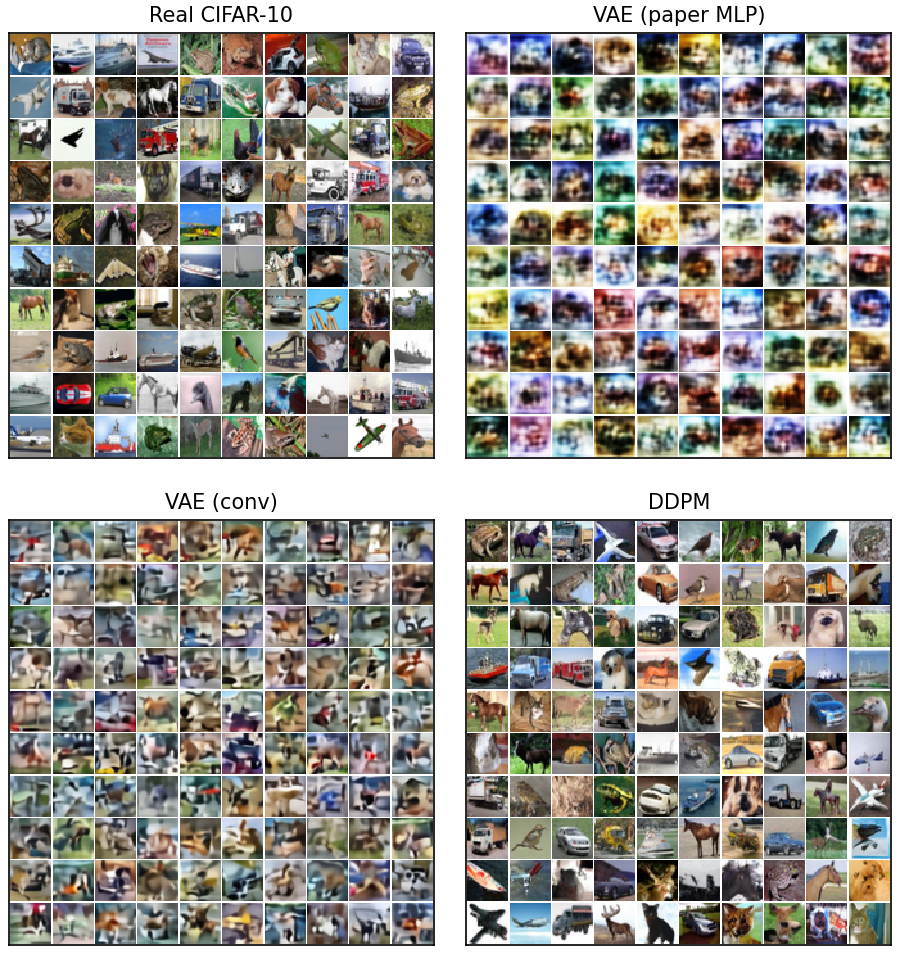
\includegraphics[width=0.86\textwidth]{fig_samples_grid.png}
\caption{Uncurated samples (first 100 of a fixed seed) of each model next to real CIFAR-10 test images.}
\label{fig:samples}
\end{figure}

\subsection{Realism}
\begin{itemize}
  \item \textbf{DDPM.} Most samples are sharp, coherent photographs with recognisable objects (horses, cars,
        trucks, ships, birds, frogs), plausible lighting and backgrounds, and correct global structure. Failures
        occur at the level of objects (implausible shapes, objects blending into the background, ambiguous
        species), while low-level texture is almost always realistic.
  \item \textbf{VAE-Conv.} Samples have plausible colours and rough layouts, typically a foreground blob on a
        background, but no sharp edges or texture.
  \item \textbf{VAE-MLP.} Samples are blurrier still: high-contrast colour blobs with little object structure.
\end{itemize}
The mechanism follows from \cref{eq:vae-recon}. The decoder models pixels as independent Gaussians, so when many
sharp images are compatible with one latent, the optimal mean is their \emph{average}, which is blurry. Each
reverse step of the DDPM, in contrast, only removes a small amount of noise. That is a nearly Gaussian problem
which a Gaussian transition models accurately, so detail survives.

\begin{figure}[H]
\centering
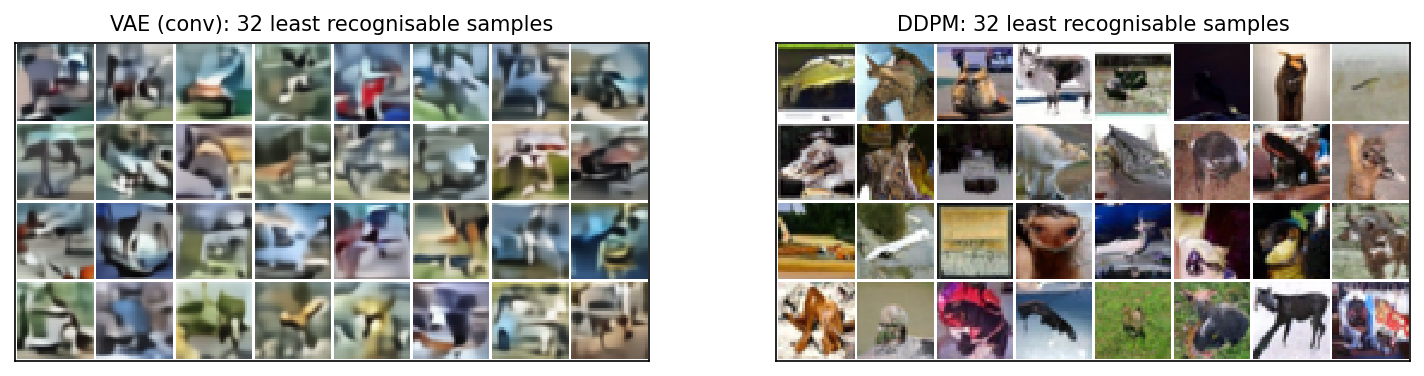
\includegraphics[width=\textwidth]{fig_failures.png}
\caption{The 32 least recognisable samples according to the classifier. The VAE's worst samples are abstract and
blurry. The DDPM's worst samples are still sharp, photograph-like images whose \emph{content} is ambiguous, as in
many real CIFAR-10 images.}
\label{fig:failures}
\end{figure}

\subsection{Diversity and thematic consistency}
The DDPM grid varies in class, colour, background, scale and viewpoint about as much as the real grid does
(recall $0.58$ vs.\ $0.69$). The VAE grids repeat similar muted colours and centred blobs (recall $0.07$).

\begin{figure}[H]
\centering
\begin{subfigure}[t]{0.49\textwidth}\centering
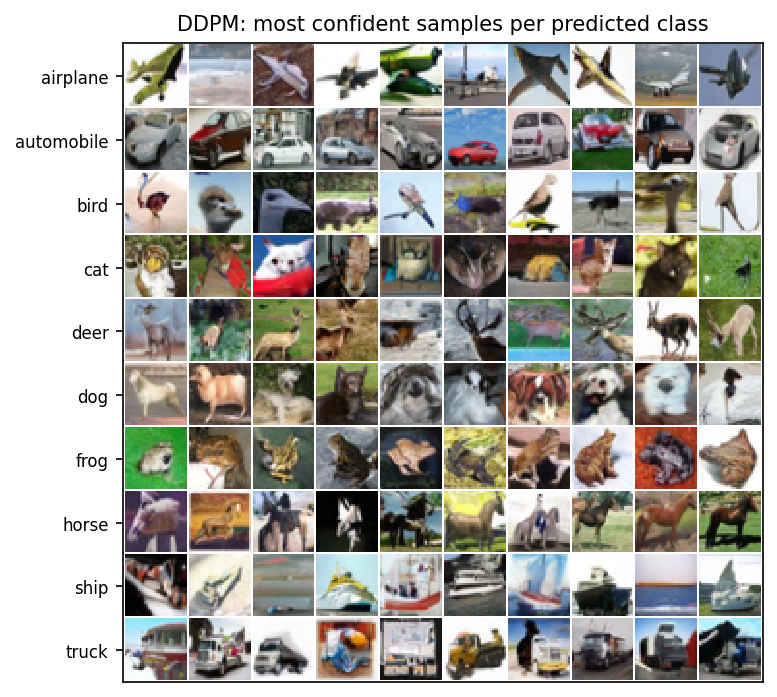
\includegraphics[width=\textwidth]{fig_by_class_ddpm_ancestral1000.png}
\caption{DDPM}
\end{subfigure}\hfill
\begin{subfigure}[t]{0.49\textwidth}\centering
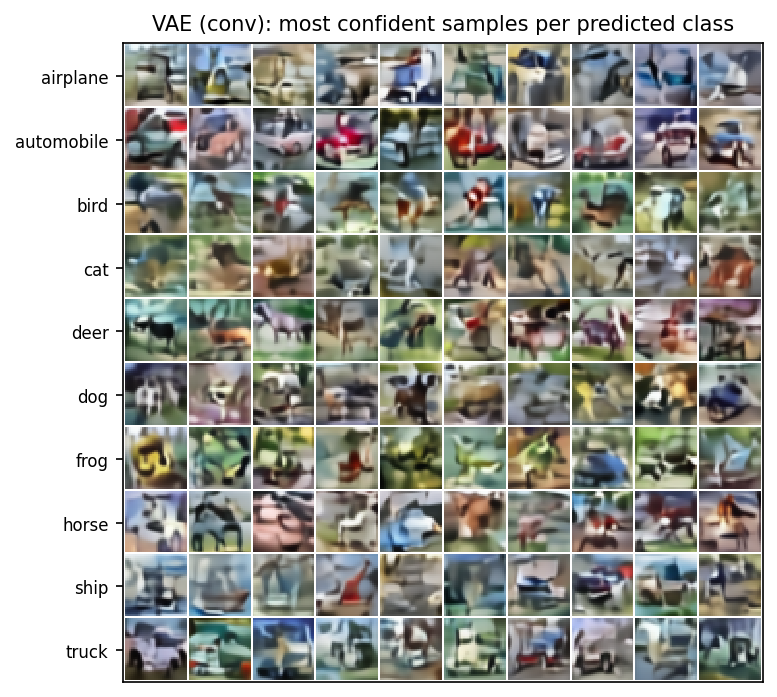
\includegraphics[width=\textwidth]{fig_by_class_vae_conv.png}
\caption{VAE-Conv}
\end{subfigure}
\caption{The classifier's most confident samples for each predicted class. DDPM samples are clear instances of
their class; even the VAE's most confident samples are only loosely related to theirs.}
\label{fig:byclass}
\end{figure}

\subsection{How each model generates}

\begin{figure}[H]
\centering
\begin{minipage}[c]{0.56\textwidth}
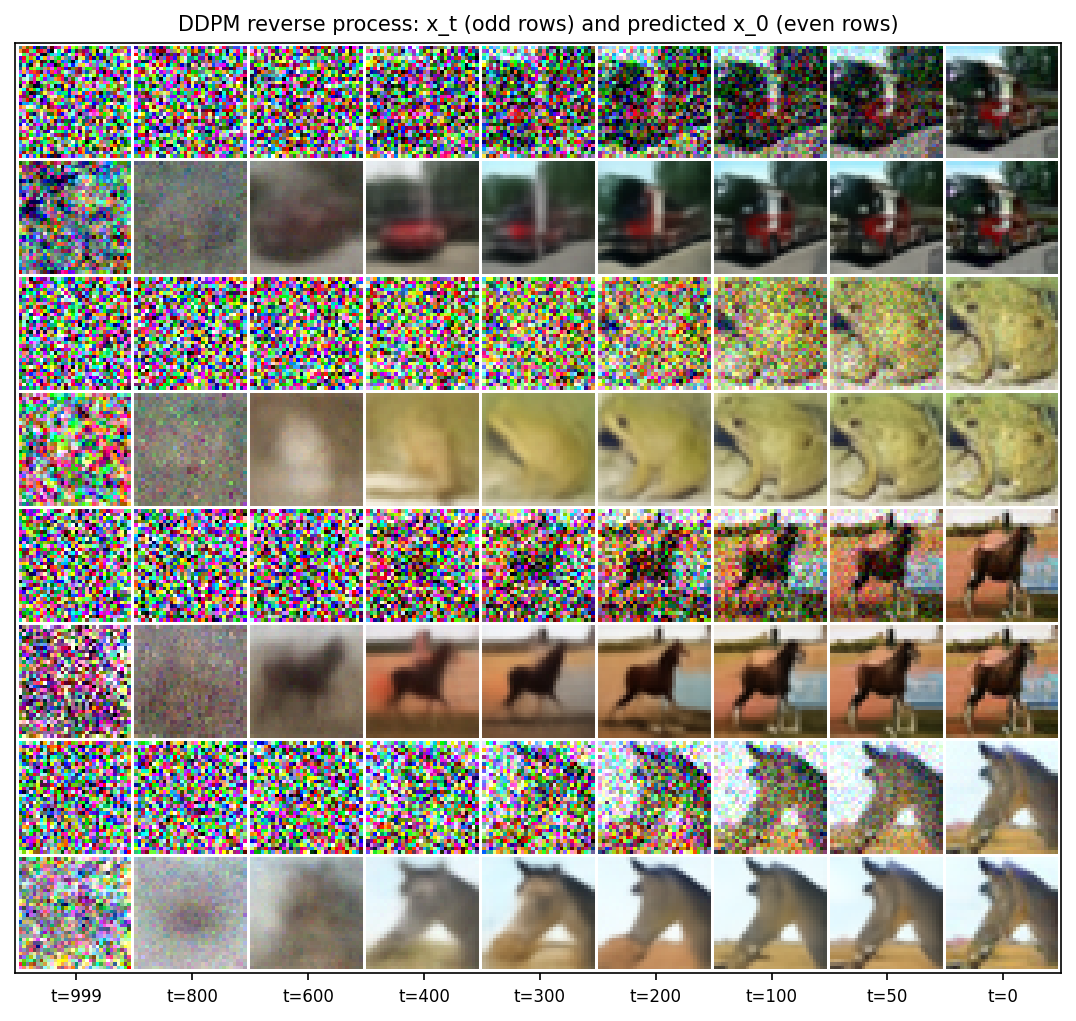
\includegraphics[width=\textwidth]{fig_ddpm_denoising.png}
\end{minipage}\hfill
\begin{minipage}[c]{0.42\textwidth}
\caption{The DDPM reverse process. Odd rows show $\x_t$ and even rows the predicted clean image $\hat\x_0$.
Generation is \emph{coarse-to-fine}: layout and colours are fixed by $t\approx600$--$400$ (a red truck, a frog, a
horse), and later steps only add detail. Together with \cref{fig:bpd}, this shows that the content is decided
early and cheaply, while most of the likelihood is spent on fine detail.}
\label{fig:denoise}
\end{minipage}
\end{figure}

\begin{figure}[H]
\centering
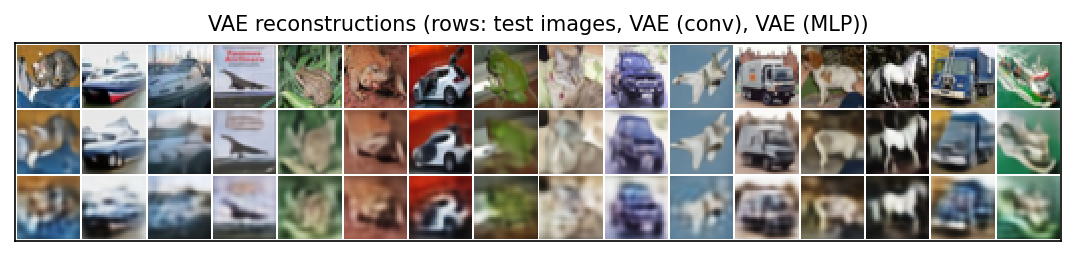
\includegraphics[width=\textwidth]{fig_vae_reconstructions.png}
\caption{VAE reconstructions. Rows: test images, VAE-Conv, VAE-MLP. Layout and colour survive the 128-d
bottleneck; texture does not.}
\label{fig:recon}
\end{figure}

The two VAEs reach almost the same PSNR ($24.07$ vs.\ $23.61$\,dB) and SSIM ($0.772$ vs.\ $0.771$) on test
reconstructions. Yet VAE-MLP's reconstructions are visibly blurrier, and their FID is far worse ($99.4$ vs.\
$57.9$). Pixel-wise metrics do not capture perceptual quality.

\subsection{Latent spaces}

\begin{figure}[H]
\centering
\begin{minipage}[c]{0.56\textwidth}
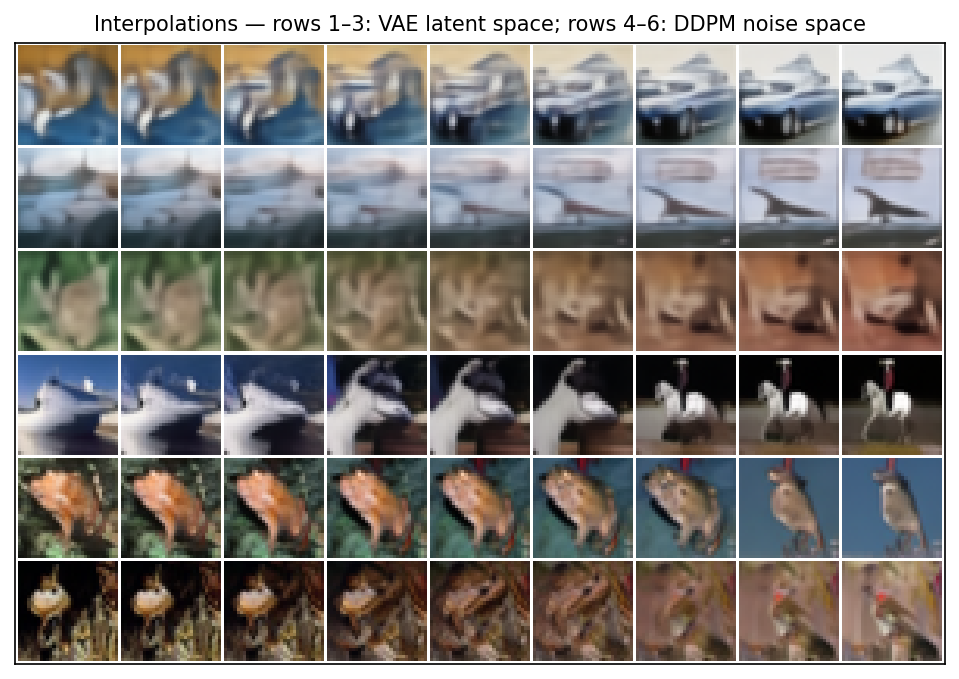
\includegraphics[width=\textwidth]{fig_interpolation.png}
\end{minipage}\hfill
\begin{minipage}[c]{0.42\textwidth}
\caption{Interpolations. Rows 1--3: linear interpolation between the VAE latents of two test images gives smooth,
gradual blends; the VAE has a learned, semantic latent space. Rows 4--6: spherical interpolation between two
DDPM starting noises $\x_T$, decoded deterministically with DDIM-50, gives sharp images throughout. The content,
however, \emph{switches} between objects rather than blending, because the DDPM's ``latent'' is simply noise.}
\label{fig:interp}
\end{minipage}
\end{figure}

\begin{figure}[H]
\centering
\begin{minipage}[c]{0.36\textwidth}
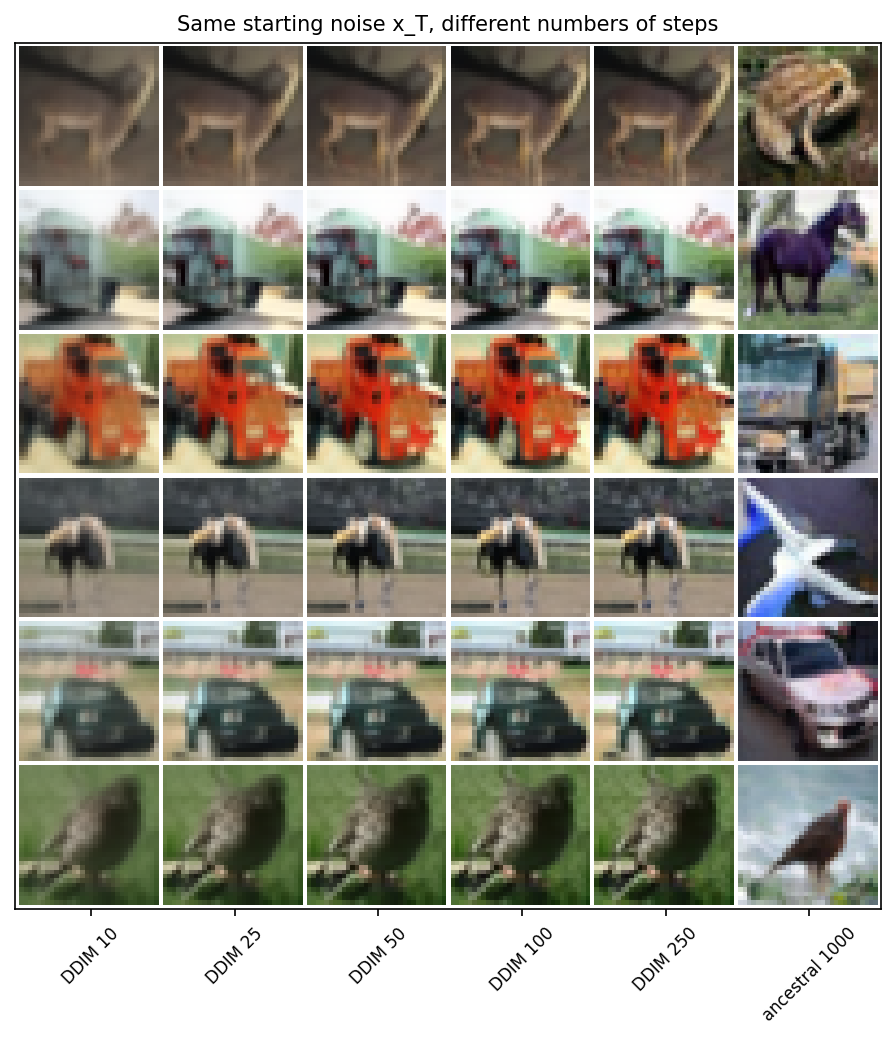
\includegraphics[width=\textwidth]{fig_ddim_steps.png}
\end{minipage}\hfill
\begin{minipage}[c]{0.6\textwidth}
\caption{The same starting noise $\x_T$ decoded with 10--250 DDIM steps, and with the 1000-step ancestral sampler
(last column). DDIM is deterministic, so every step count gives the \emph{same} image and extra steps only sharpen
details. The ancestral sampler adds fresh noise at every step, so its image differs. This is expected, not a bug.}
\label{fig:ddimsteps}
\end{minipage}
\end{figure}

\subsection{Blind rating by a vision-language model}
\label{sec:blind}

As an independent, subjective judgement, we ran a blind rating of 150 shuffled images: 50 real CIFAR-10 test
images, 50 VAE-Conv samples and 50 DDPM samples (1000-step sampler), drawn at random from the evaluated sample
sets. The rater was \textbf{Gemini}, a vision-language model, not a person. For every image it gave:
\begin{itemize}
  \item a realism score from 1 to 5;
  \item the CIFAR-10 class, or ``unrecognisable'';
  \item a verdict of real or generated.
\end{itemize}
The instructions named neither the models nor the proportions of each source, and stated that low resolution
alone is no sign of being generated.

\begin{table}[H]
\centering\small
\caption{Blind rating by Gemini (50 images per source; 95\% Wilson intervals in brackets).}
\label{tab:blind}
\begin{tabular}{@{}lcccc@{}}
\toprule
Source & Mean realism (1--5) & Named a class & Judged ``real'' & Correct class\\
\midrule
Real test images & \textbf{4.58} & 100\% & 96\% [87, 99] & 96\%\\
DDPM & 4.28 & 98\% & \textbf{96\% [87, 99]} & --\\
VAE-Conv & 1.34 & 24\% & 0\% [0, 7] & --\\
\bottomrule
\end{tabular}
\end{table}

\begin{itemize}
  \item \textbf{Gemini could not tell DDPM samples from real photographs.} It judged 48 of 50 in each group to be
        real, so its real-vs-DDPM accuracy is $50\%$, i.e.\ chance.
  \item \textbf{Its graded scores still detect a small gap.} Realism averaged $4.28$ for DDPM vs.\ $4.58$ for real
        photos (Mann--Whitney $p=0.015$), consistent with the remaining FID gap.
        DDPM samples also received fewer top scores of 5 (20 vs.\ 33 of 50).
  \item \textbf{Every VAE sample was identified as generated.} 33 of the 50 VAE samples received the lowest
        realism score, and only $24\%$ could be assigned any class, independently confirming \cref{tab:thematic}.
  \item \textbf{Almost all DDPM samples were recognisable} ($98\%$ were assigned a class), and Gemini's labels cover
        all ten classes.
\end{itemize}

\paragraph{Integrity.} All 50 ``real'' images are exact CIFAR-10 test images with the labels in the answer key, and
none of the 100 generated images appears in the test set. The rater's answers contradict the key exactly where a
blind rater would err: it labelled 48 of 50 DDPM samples ``real''. We report this single automated rater as
supporting evidence, not as a substitute for a human study.
